\section{Theorie}
\label{sec:Theorie}
\subsection{Komplexe Widerstände}
Bevor die Brückenschaltungen im Einzelnen betrachtet werden, muss zwischen verschiedenen Formen von elektrischen Widerständen -- 
auch \textit{Impedanzen} -- unterschieden werden. 

Neben den ohmschen Widerständen $R$ sorgen auch Spulen mit der Induktivität $L$ und Kondensatoren mit der Kapazität $C$, 
die sich mit im Stromkreis befinden, für eine Veränderung des Strom- und Spannungsverhalten. 
Der ohmsche Widerstand sorgt für einen Spannungsabfall von 
\begin{equation}
    U=RI .
    \label{eqn:ohm}
\end{equation}
Kondensatoren und Spulen hingegen bewirken zusätzlich eine Phasenverschiebung des Wechselstroms und der Wechselspannung,
die den Stromkreis betreiben. 
In der reellen Schreibweise mit trigonometrischen Funktionen recht kompliziert, vereinfacht sich die Darstellung dessen 
mit komplexen Zahlen: 
Ohmsche sowie induktive und kapazitive Widerstände werden zu einer komplexwertigen Impedanz zusammengefasst. 
Dabei stellen letztere beiden den Imaginäranteil dar, wodurch die Phasenverschiebung algebraisch umgesetzt wird. 
Da sie in dem Sinne keinen effektiven Spannungsabfall bewirken, sind sie auch unter dem Namen \textit{Scheinwiderstand} geläufig.
Somit hat die Impedanz $Z$ von den drei in Reihe geschalteten Widerständen die Form 
\begin{equation}
    Z = R + \symup{i}\omega L - \symup{i}\frac{1}{\omega C} ,
    \label{eqn:impedanz}
\end{equation}
wobei $\omega$ die Kreisfrequenz der angelegten Wechselspannung $\tilde{U} = \hat{U} \symup{e}^{\symup{i}\omega t}$ ist.
Mit der komplexen Impedanz kann wie mit dem ohmschen Widerstand in \eqref{eqn:ohm} die Spannung und der Strom berechnet werden. 

\subsection{Die Kirchhoff'schen Gesetze}
Das erste Gesetz, ebenfalls unter der Knotenregel bekannt, leitet sich aus der Ladungserhaltung ab. 
An einem Knoten in einem Stromkreis muss die Summe der zufließenden Ströme gleich der der abfließenden sein. 
Definiert man eine entsprechende Vorzeichenregelung (z.B. alle abfließenden Ströme sind positiv, alle zufließenden negativ) 
erhält man den Ausdruck: 
\begin{equation}
    \sum_k I_k .
    \label{eqn:kirchhoff1}
\end{equation}

Das zweite Gesetz beruft sich auf die Energieerhaltung und die Existenz eines eindeutigen elektrischen Potentials. 
Als Folgerung daraus ergibt sich die sogenannte Maschenregel, die 
\begin{equation}
    \sum_k U_k
    \label{eqn:kirchhoff2}
\end{equation}
innerhalb eines geschlossenen Leiters -- also einer Masche -- postuliert. 
Dabei sind die Spannungsquellen und -abfälle $U_k$ jeweils mit einem entsprechenden Vorzeichen versehen, je nachdem, ob sie 
in gleicher oder verschiedener Richtung gepolt sind. 

\subsection{Brückenschaltungen}
\begin{figure}
    \centering
    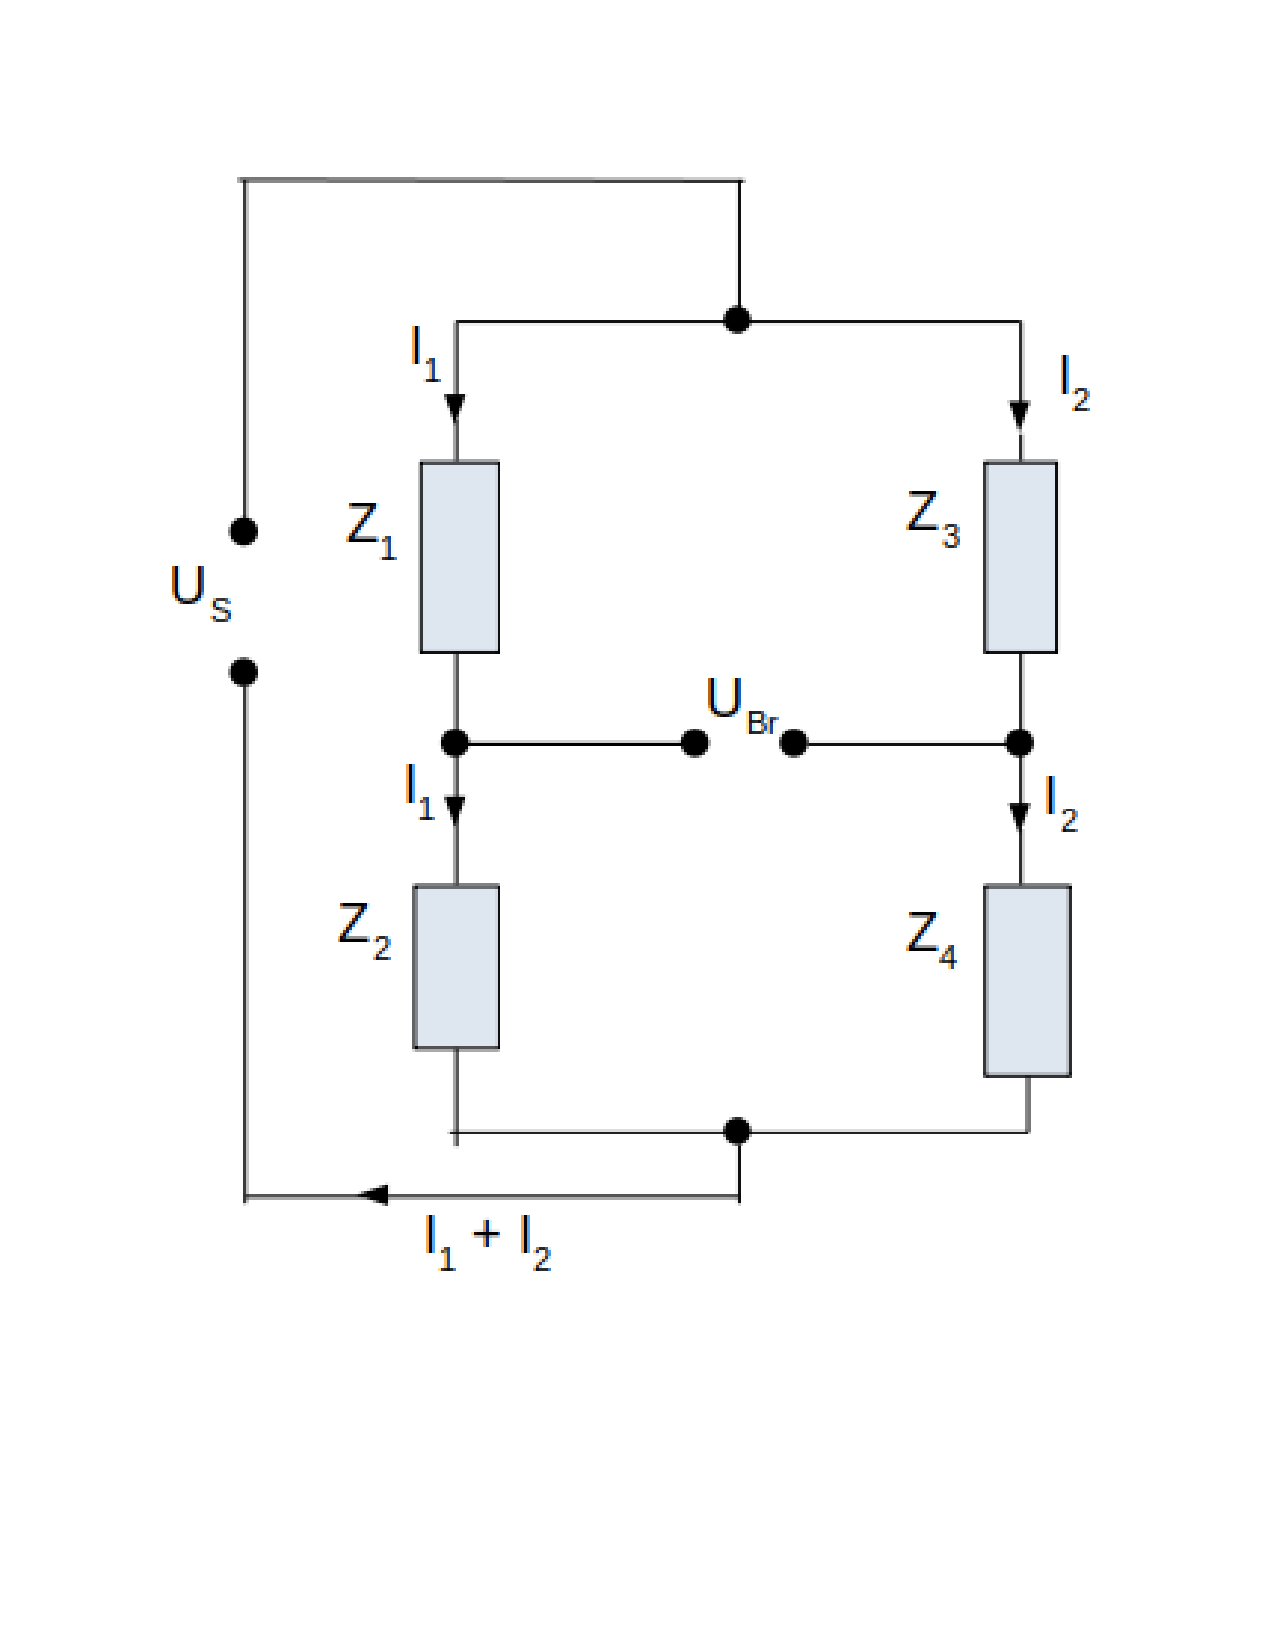
\includegraphics[width=0.5\textwidth]{Schaltung1.pdf}
    \caption{Eine allgemeine Brückenschaltung.}
    \label{fig:allg_schalt}
\end{figure}

\subsubsection{Wheatstone'sche Brückenschaltung}